\documentclass{sigchi}

% Use this section to set the ACM copyright statement (e.g. for
% preprints).  Consult the conference website for the camera-ready
% copyright statement.

% Copyright
\CopyrightYear{2020}
%\setcopyright{acmcopyright}
\setcopyright{acmlicensed}
%\setcopyright{rightsretained}
%\setcopyright{usgov}
%\setcopyright{usgovmixed}
%\setcopyright{cagov}
%\setcopyright{cagovmixed}




% Use this command to override the default ACM copyright statement
% (e.g. for preprints).  Consult the conference website for the
% camera-ready copyright statement.

%% HOW TO OVERRIDE THE DEFAULT COPYRIGHT STRIP --
%% Please note you need to make sure the copy for your specific
%% license is used here!
% \toappear{
% Permission to make digital or hard copies of all or part of this work
% for personal or classroom use is granted without fee provided that
% copies are not made or distributed for profit or commercial advantage
% and that copies bear this notice and the full citation on the first
% page. Copyrights for components of this work owned by others than ACM
% must be honored. Abstracting with credit is permitted. To copy
% otherwise, or republish, to post on servers or to redistribute to
% lists, requires prior specific permission and/or a fee. Request
% permissions from \href{mailto:Permissions@acm.org}{Permissions@acm.org}. \\
% \emph{CHI '16},  May 07--12, 2016, San Jose, CA, USA \\
% ACM xxx-x-xxxx-xxxx-x/xx/xx\ldots \$15.00 \\
% DOI: \url{http://dx.doi.org/xx.xxxx/xxxxxxx.xxxxxxx}
% }

% Arabic page numbers for submission.  Remove this line to eliminate
% page numbers for the camera ready copy
% \pagenumbering{arabic}

% Load basic packages
\usepackage{balance}       % to better equalize the last page
\usepackage{graphics}      % for EPS, load graphicx instead 
\usepackage[T1]{fontenc}   % for umlauts and other diaeresis
\usepackage{txfonts}
\usepackage{mathptmx}
\usepackage[pdflang={en-US},pdftex]{hyperref}
\usepackage{color}
\usepackage{booktabs}
\usepackage{textcomp}

% Some optional stuff you might like/need.
\usepackage{microtype}        % Improved Tracking and Kerning
% \usepackage[all]{hypcap}    % Fixes bug in hyperref caption linking
\usepackage{ccicons}          % Cite your images correctly!
% \usepackage[utf8]{inputenc} % for a UTF8 editor only

% If you want to use todo notes, marginpars etc. during creation of
% your draft document, you have to enable the "chi_draft" option for
% the document class. To do this, change the very first line to:
% "\documentclass[chi_draft]{sigchi}". You can then place todo notes
% by using the "\todo{...}"  command. Make sure to disable the draft
% option again before submitting your final document.
\usepackage{todonotes}

% Paper metadata (use plain text, for PDF inclusion and later
% re-using, if desired).  Use \emtpyauthor when submitting for review
% so you remain anonymous.
\def\plaintitle{SIGCHI Conference Proceedings Format}
\def\plainauthor{First Author, Second Author, Third Author,
  Fourth Author, Fifth Author, Sixth Author}
\def\emptyauthor{}
\def\plainkeywords{Authors' choice; of terms; separated; by
  semicolons; include commas, within terms only; this section is required.}
\def\plaingeneralterms{Documentation, Standardization}

% llt: Define a global style for URLs, rather that the default one
\makeatletter
\def\url@leostyle{%
  \@ifundefined{selectfont}{
    \def\UrlFont{\sf}
  }{
    \def\UrlFont{\small\bf\ttfamily}
  }}
\makeatother
\urlstyle{leo}

% To make various LaTeX processors do the right thing with page size.
\def\pprw{8.5in}
\def\pprh{11in}
\special{papersize=\pprw,\pprh}
\setlength{\paperwidth}{\pprw}
\setlength{\paperheight}{\pprh}
\setlength{\pdfpagewidth}{\pprw}
\setlength{\pdfpageheight}{\pprh}

% Make sure hyperref comes last of your loaded packages, to give it a
% fighting chance of not being over-written, since its job is to
% redefine many LaTeX commands.
\definecolor{linkColor}{RGB}{6,125,233}
\hypersetup{%
  pdftitle={\plaintitle},
% Use \plainauthor for final version.
%  pdfauthor={\plainauthor},
  pdfauthor={\emptyauthor},
  pdfkeywords={\plainkeywords},
  pdfdisplaydoctitle=true, % For Accessibility
  bookmarksnumbered,
  pdfstartview={FitH},
  colorlinks,
  citecolor=black,
  filecolor=black,
  linkcolor=black,
  urlcolor=linkColor,
  breaklinks=true,
  hypertexnames=false
}

% create a shortcut to typeset table headings
% \newcommand\tabhead[1]{\small\textbf{#1}}

% End of preamble. Here it comes the document.
\begin{document}

\title{3D EMOTION GAN: EMOTION-DRIVEN GAN AS AN INPUT METHOD FOR CREATING 3D ART FORMS}

\numberofauthors{3}
\author{%
  \alignauthor{Kellyn Dassler\\
    \affaddr{Colorado State University}\\
    \affaddr{Fort Collins, Colorado}\\
    \email{kellyndassler@gmail.com}}\\
}

\maketitle

\begin{abstract}
We propose a method for generating three dimensional objects from emotion-based two-dimensional image inputs via a two-step neural network process. Using an auxiliary classifier generative adversarial neural network framework with a 2D-to-3D style transfer neural network, we create novel three-dimensional objects driven by emotion-based art and user-provided emotion selection. Preliminary results show that our process generates objects that exhibit psychologically-based emotional features, and initial user studies reveal that this process may provide a new way for users to imbue personal emotions into 3D virtual objects and art.
\end{abstract}

% Author Keywords
\keywords{generative adversarial networks, three-dimensional neural style transfer, three-dimensional art, emotion-driven art, auxiliary classifier generative adversarial neural network}

\section{Introduction}

Art psychologically reflects its creator’s emotions \cite{AlvarezMelis2017TheEG}. Similarly, art therapy, occupational therapy, and other mental health interventions utilize creative expression to regulate and improve emotional regulation \cite{article}. However, many of these interventions are cost-prohibitive, difficult for users to pick-up quickly, and only accessible to limited populations \cite{article}. Virtual art forms provide an artistic medium that addresses the aforementioned issues, but many users still feel intimidated by the creative process \cite{article}. While several studies have proposed methods for allowing users to generate two-dimensional images that reflect human emotions using generative adversarial networks \cite{AlvarezMelis2017TheEG}, none have studied methods for generating emotionally reflective three-dimensional forms. Thus, through this study, we seek new user access points to three-dimensional art creation via co-creative design techniques with artificially intelligent neural networks.

\section{Related Work}

\subsection{GANs}
Generative Adversarial Networks (GANs) were proposed in 2014 as a two network model to generate novel data from pre-existing data \cite{goodfellow2014generative}. They consist of at least one generator network and one discriminator network that are simultaneously trained in an adversarial fashion. For image data in particular, the generator creates increasingly improved novel data by testing generated images against the discriminator, which determines whether the generated image is ‘real’ or ‘fake’ \cite{goodfellow2014generative}.  As the discriminator is trained, its accuracy increases until the generator creates images that highly mirror the initial dataset \cite{goodfellow2014generative}. This flagship paper outlined the initial GAN framework, which has since been extended and improved upon in architectures like conditional GANs, collaborative GANs, and deep convolutional GANs  \cite{acgan}.

\subsection{Neural Style Transfer}
Shortly after GANs debuted, Leon and colleagues proposed a method of transferring the art style of one image to the content of another image using biologically inspired deep neural networks \cite{Gatys_2016}. By separating intermediate layer activations that represent artistic features like edges, textures, color, and shape from a convolutional image classification network, network creators can generalize these features and apply them to any other image with novel content \cite{Gatys_2016}. Although this is a neural network-based approach, it is not generative in the true sense of creating completely novel outputs. 

\subsection{Emotional GAN}
Created by MIT Media Lab members in 2017, the Emotional GAN uses a modified conditional GAN with an extensive WikiArt and MOMA artwork dataset to generate novel images that represent human emotions \cite{AlvarezMelis2017TheEG}. They took an independent approach to dataset creation by recruiting annotators to indicate the emotion most invoked in them by the image. They achieved state-of-the-art results for emotion-based image creation, and generated novel images in six different categories—anger, anxiety, fear, joy, sadness, and neutral. Although they created artwork that exhibited emotional features reflective of relevant psychological and artistic literature, they did not study the application of this framework to user creative expression.

\subsection{3D Object Generation}
Liu, Yu, and Funkhouser showed how novice users can create interactive three-dimensional shapes through a voxel model interface connected to an iterative GAN \cite{Liu_2017}. By applying a latent vector to a 3D voxel model created by the user alongside an iterative GAN and SNAP processing pipeline, users can generate a more realistic shape from the input \cite{Liu_2017}. Their research argues that GANs can provide a process through which users with no formal art training can participate in computer-assisted interactive modeling \cite{Liu_2017}, but it does not address creative forms of expression and human-GAN co-creation. 

\section{Methodology}

\subsection{Method of Emotional Transfer via Two-Step Neural Network Process}
The emotion-to-three-dimensions framework was facilitated through a two-step neural network process. Initially, we trained an auxiliary classifier generative adversarial neural network (AC-GAN) using an emotion-labeled two-dimensional artwork dataset. After training, the AC-GAN was able to successfully create plausible novel artwork images reflecting major human emotions, including happiness, fear, anger, sadness, and anxiety. To use these images as novel input for creating three-dimensional objects, users were given a Jupyter notebook-based application through which they indicated their emotions and altered the generated photos before sending the photos to a 2D-to-3D neural transfer style network. In a preliminary user preference study, the participants were trained in both manual three-dimensional object creation using a polybrush in Unity3D as shown in \emph{Figure 1}, and the two-step neural network object creation process as shown in \emph{Figure 2}. After creating objects for each major emotion through both approaches, the users’ indicated their preferred creation method and produced outputs for each emotion. Finally, we interviewed each user to gather qualitative preference data to provide insight into user preferences. 

\begin{figure*}
  \centering
  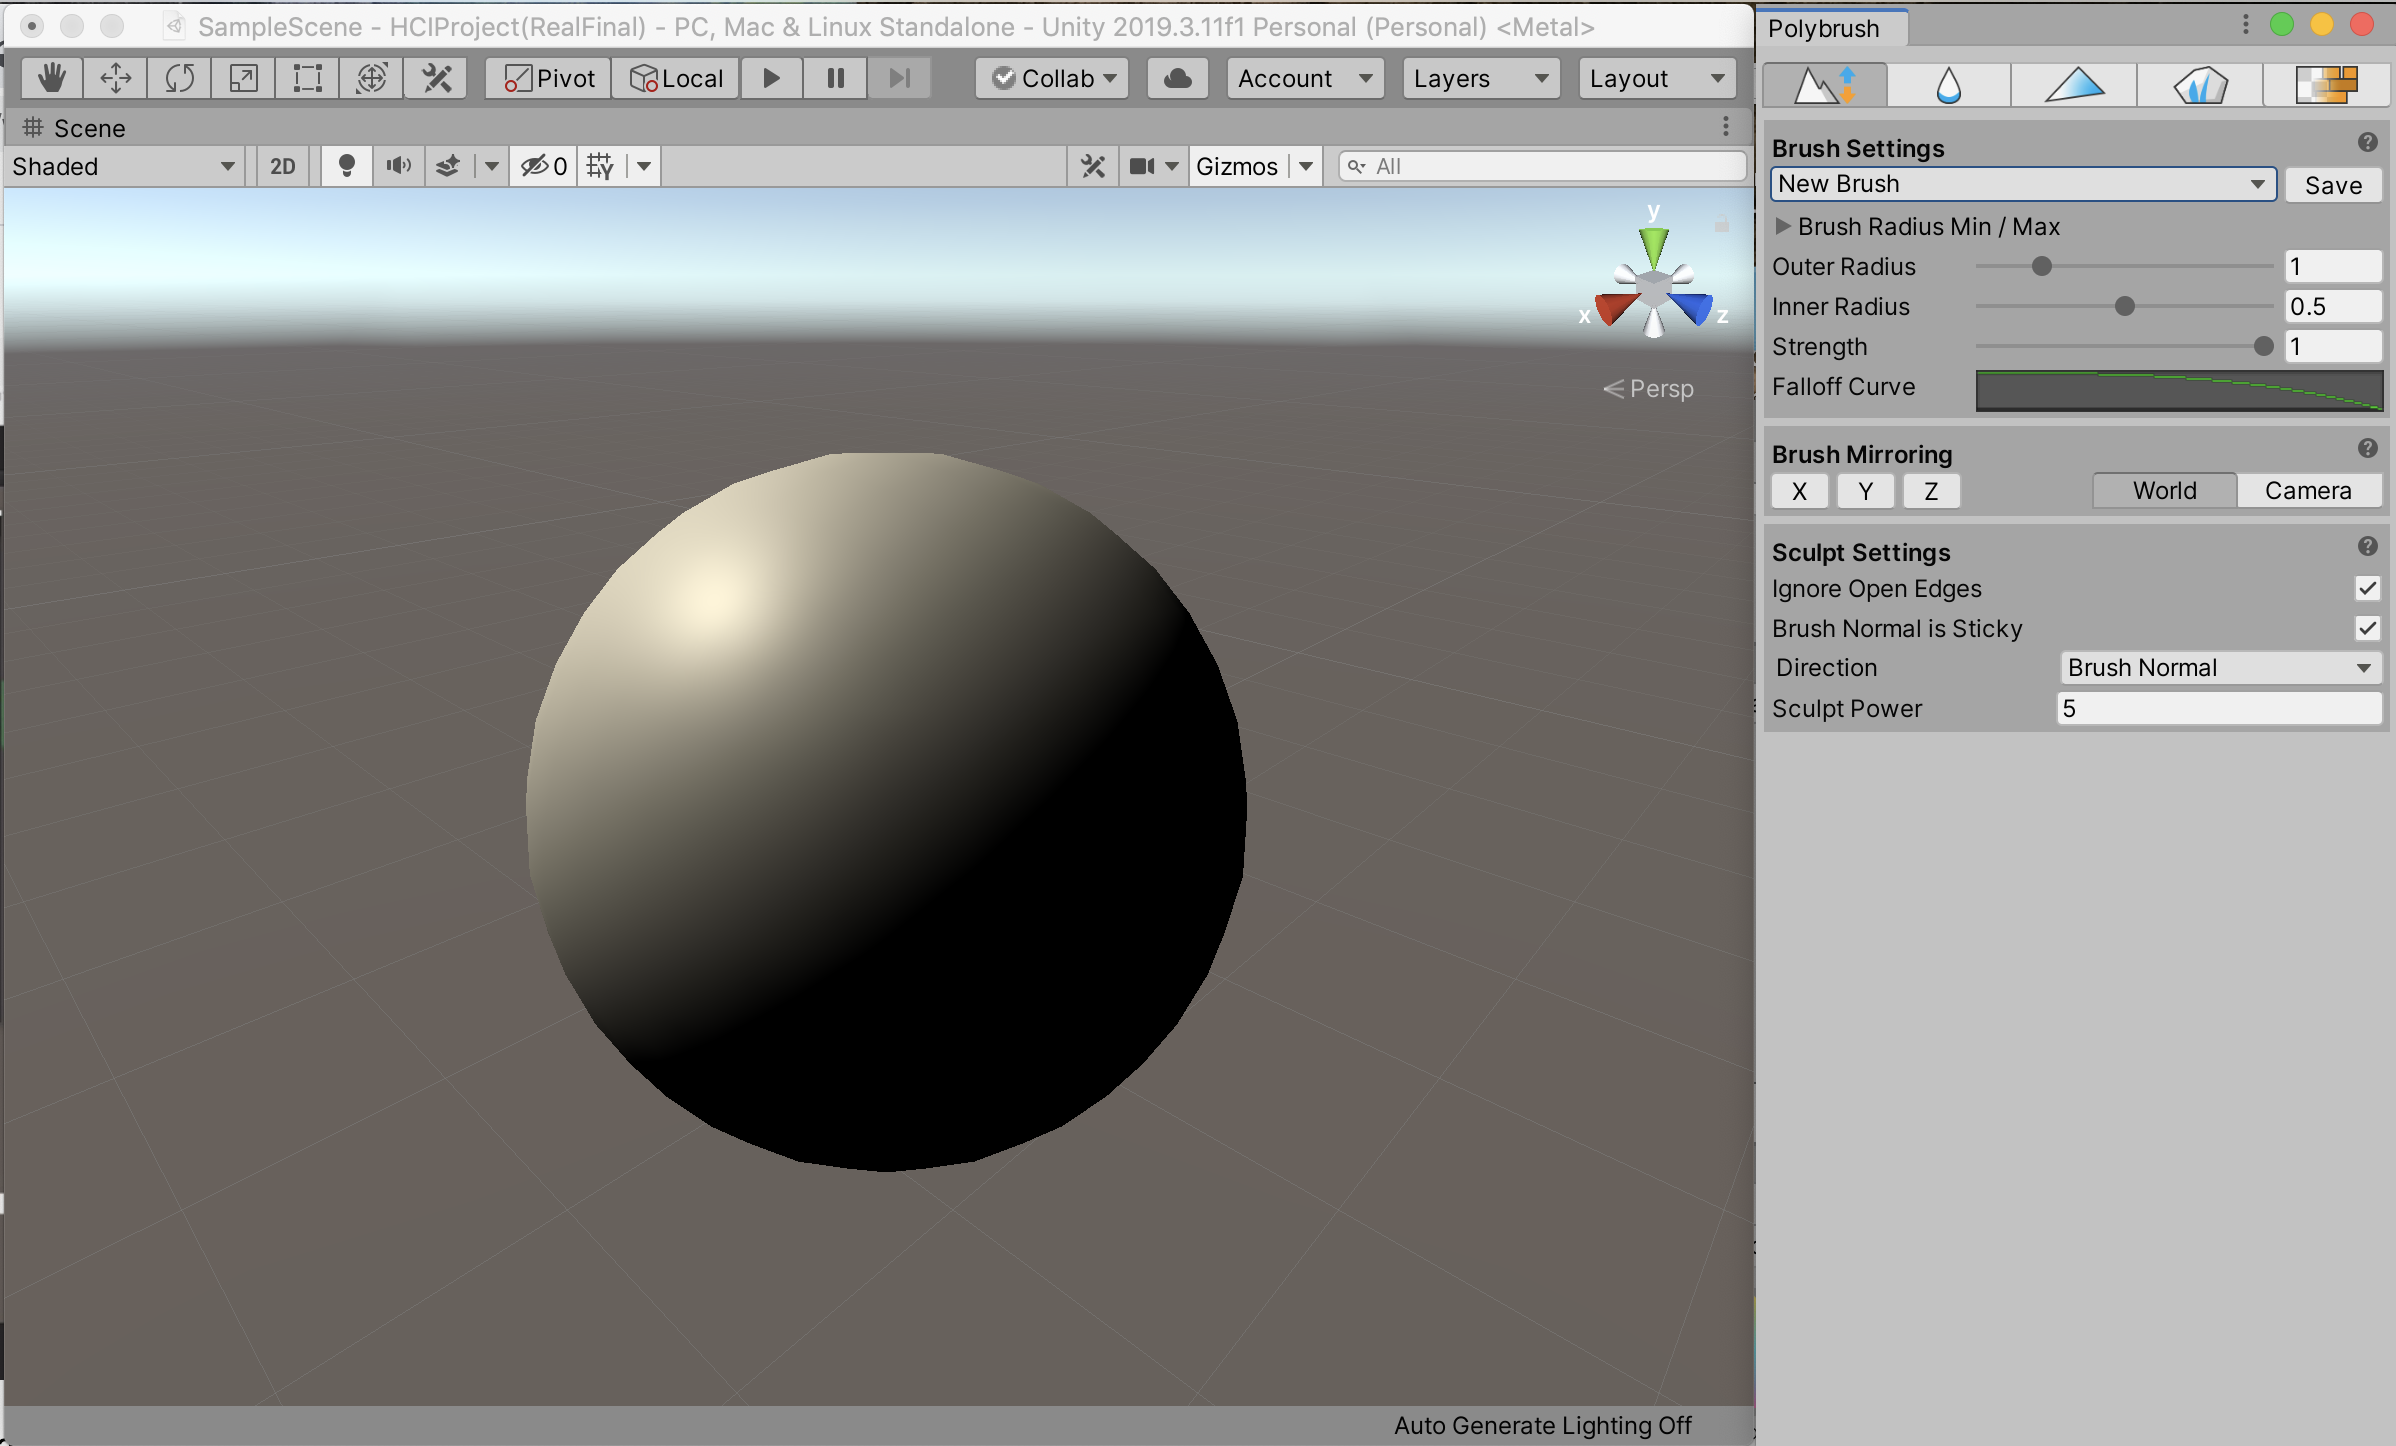
\includegraphics[width=2\columnwidth]{figures/polybrushstart}
  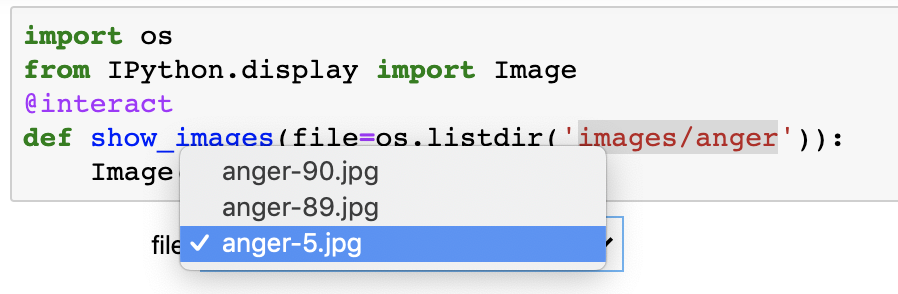
\includegraphics[width=2\columnwidth]{figures/selection}
  \caption{Polybrush process initial setup in Unity3D.}~\label{fig:figure1}
\end{figure*}

\subsection{Dataset Characterization}
The generated style images are rooted in an emotion-labeled artwork dataset processed from the original WikiArt artwork database and annotated with human emotions garnered from ten or more annotators, available from the WikiArt Emotions Dataset webpage \cite{LREC18-ArtEmo}. Each image was accompanied by floating point values that indicated the value of 20 different emotions present in the image. In total, 2865 annotated images were downloaded using support from the pandas Python package. To retrieve the major emotion most expressed by each image, we eliminated emotions that did not match one of five emotion categories-- happiness, fear, anger, sadness, and anxiety—and then processed the dataset to find the maximum value amongst the remaining emotion categories. These emotions were chosen due to their straightforward nature and consistency among users and high levels of representation within the dataset. Each image was then loaded into an image array and resized to 28x28 pixels, while each corresponding emotion label was processed into a label list to prepare the data for network training.

The content object files were created via object files using XCode with additional provided object files from the neural renderer repository. While we included objects other than spheres for future work, we only utilized the sphere object to run the study, in order to account for constraints and confounding variables. These were imported into the data examples directory for use by the transfer style neural network.

\subsection{AC-GAN}
GANs are an artificially intelligent architecture for creating novel data from existing inputs \cite{goodfellow2014generative}. Conditional GANs, a deep convolutional subset of traditional GANs used for creating images, use class-labeled image input to create images of one or more chosen types \cite{10.5555/3305890.3305954}. The AC-GAN extends the generative process of the conditional GAN by adding a class label prediction into the discriminator network, which allows the network to create novel images and determine which class they fit into best \cite{10.5555/3305890.3305954}. This alteration stabilizes network training to produce higher quality image representations in the latent space \cite{acgan}. This structure is well-suited to our proposed method because it allows each generated output to be novel exhibit learned attributes indicative of a given emotion class. 

The traditional GAN architecture consists of two networks with shared model weights—a generator and a discriminator. While the generator takes in random noise from a given latent space to produce images, a discriminator classifies the images as either dataset-based (‘real’) or generated (‘fake’) \cite{acgan}. Both networks are trained simultaneously until the discriminator can no longer detect if a generated image is ‘real’ or ‘fake’. The ACGAN model extends this framework through latent space structure, class label input to the generator, and an added class prediction function in the discriminator \cite{10.5555/3305890.3305954}, as shown in the graph from the authors in \emph{Figure 3}. In this architecture, the generator is given a point in latent space and a class label as input, rather than random noise. Then, it must generate an image that reflects features of the given class \cite{10.5555/3305890.3305954}. In contrast, the discriminator is given an image and must predict both the genuineness of the data and a class label \cite{acgan}. In our model, this is determined through a sigmoid activation function, which determines the probability that an image is ‘real’, and a SoftMax activation function, which outputs the probability that an image belongs to each class. The sigmoid activation function is optimized via binary cross entropy, while the SoftMax activation function is optimized through categorical cross entropy as suggested by the flagship AC-GAN paper \cite{10.5555/3305890.3305954}, and both networks are trained to maximize probabilities for both functions. For example, in our WikiArt emotions dataset, the generator might conditionally generate an image for the emotion class “angry” that reflects the jagged shapes, red and black colors, and rough textural features typical of other “angry” labeled images. Then, the discriminator attempts to distinguish whether this output is valid and predict which emotion class it fits into best. If enough of features of the generated image reflects those of the “angry” category, then the discriminator will likely correctly predict its class as “angry”. After extensive training, this model produces plausible novel images that represent the features of each class. 

\begin{figure*}
  \centering
  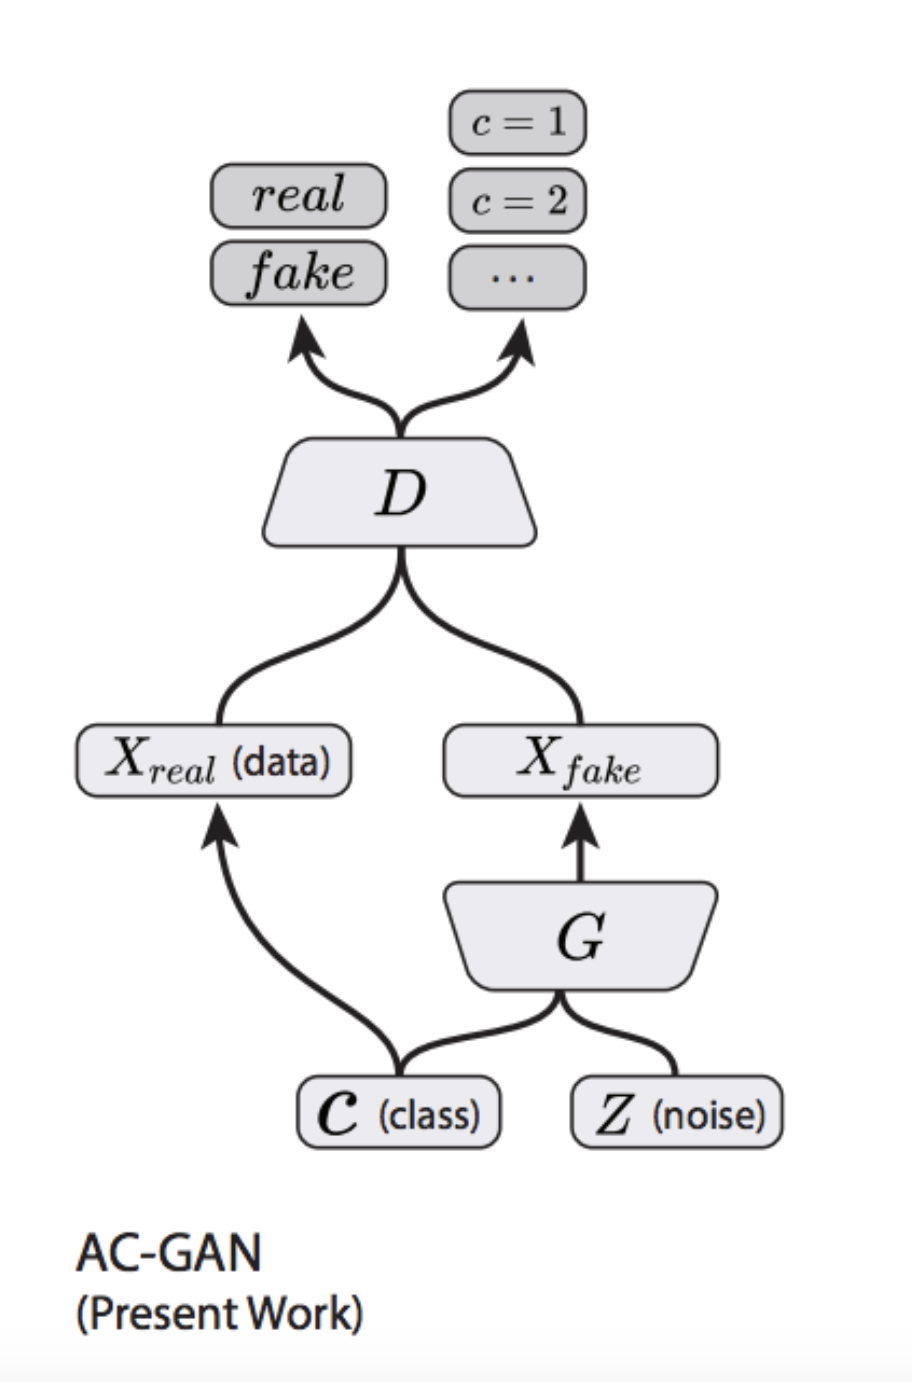
\includegraphics[width=2\columnwidth]{figures/ACGAN}
  \caption{ACGAN architecture summary.}~\label{fig:figure3}
\end{figure*}

\subsection{Neural Transfer 2D-to-3D Mesh Renderer}
In contrast to traditional GANs, neural style transfer networks apply the features of a single image input to an unrelated output, rather than generating entirely novel data \cite{neuraltrans}. In the original style transfer algorithm, a style image is applied to a content image using a pretrained VGG19 network architecture for image classification, deconstructed into layers that are used to define the image contents and styles \cite{neuraltrans}. For our proposed method, we used a pre-trained 2D-to-3D mesh renderer network for image style transfer \cite{DBLP:journals/corr/abs-1711-07566}to three-dimensional objects called Neural Renderer \cite{DBLP:journals/corr/abs-1711-07566}. To convert an image into a polygon object mesh, the network utilizes an approximate gradient approach for rasterization to enable a rendering component in the network. Thus, the network can circumvent the usual prevention of backpropagation by rasterization and create three-dimensional mesh reconstructions that reflect the shape, color, and texture of the two-dimensional input image. According to the flagship neural renderer paper, this mesh reconstruction process outperforms existing voxel-based approaches \cite{DBLP:journals/corr/abs-1711-07566}.

\subsection{Network Training Process}
We trained our AC-GAN model with Google CoLab’s TPU hardware, written in Python on a TensorFlow core using eighty percent of the class-labeled image data for a total of 2292 images. The generator model was implemented using the class label as an embedded feature map and interpreting the latent space point with a full connected layer to create 7x7 feature maps for image generation. Then, the feature maps were upscaled twice to reach a 28x28 size using a ReLU activation function, as suggested by the flagship paper \cite{10.5555/3305890.3305954}. The discriminator model was defined with an altered DCGAN architecture, featuring Gaussian weight initialization, batch normalization, Leaky ReLU, Dropout, and a 2x2 down sampling stride. Each output layer was initialized using the appropriate sigmoid activation function or SoftMax activation function for novelty and class probabilities. Both activation functions were also optimized using the associated pre-defined Keras loss functions—binary cross entropy, and categorical cross entropy. The two models were combined and optimized using an Adam optimizer with a learning rate of 0.0002 and B1 of 0.5. Each input image was pre-processed to 28x28 pixel images and the model generated novel image outputs for each emotion class— happiness, fear, anger, sadness, and anxiety. Following training, the images were validated and tested using the remaining twenty percent of image data. Generated images were analyzed for psychologically-based emotional feature representation, as described in the Emotion GAN paper \cite{AlvarezMelis2017TheEG}, and then displayed and stored for later use. 

For the next part of the study, a pre-trained 2D-to-3D neural renderer \cite{DBLP:journals/corr/abs-1711-07566} was used to convert the generated two-dimensional images into three-dimensional object meshes. This adapted code was built in Python and TensorFlow and used an approximate gradient for rasterization operations to prevent back-propagation \cite{DBLP:journals/corr/abs-1711-07566}. It also employed a content loss and style loss function for feature extraction and Gram matrix vector transformation. This network was run for each selected emotion during the user study using user-selected generated image data from the AC-GAN network as the style and a sphere object as the content. Each stylized object reflected the shape, color, and texture of the user-selected generated image. 

\subsection{User Preference Study}
To test our proposed creative method, we conducted a user preference study among six participants. The study was comprised of two creation input conditions: a Unity3D polybrush virtual object creation process (hereafter referred to as the polybrush process) and our three-dimensional emotion GAN virtual object creation process (hereafter referred to as the emotion GAN process). Each participant created objects through both processes for each of the five emotions---- happiness, fear, anger, sadness, and anxiety. The process creation order was randomized for each user. To reduce confounding variables, none of the selected participants had previous experience with Unity3D or artificial intelligence co-creation techniques. Additionally, each participant was given an initial questionnaire that asked about their comfort levels with art creation, how strongly they felt their emotions, and whether or not they tend to express their emotions through creative outlets such as art, music, or writing.

For the polybrush process, participants were given 25 minutes to learn basic rotation commands and polybrush maneuvers for altering shape, color, and texture of a given object in Unity3D. They were each shown the “Polybrush Introduction and Tutorial” available on Unity3D’s website \cite{polybrush}. Then they were given an additional 5 minutes to practice polybrush techniques on a sphere object as shown in Figure 1. The polybrush tool was set to utilize open edges and a sticky brush technique among all users and they were allowed to alter shape, texture, color, and smoothing of their given structure. For ease of use and some issues with color painting during initial test runs, users were also given the option to add a single-color material to their object instead of painting it and the accompanying directions. After practicing polybrush maneuvers, the users were given a sphere-shaped virtual object in the Unity platform and were asked to produce a three-dimensional object that reflected their understanding of one of the five selected major human emotions. Each emotion was randomized for each participant. The participant was then given 10 minutes to create and finish their virtual sculpture. This was repeated for each of the five emotions, and each virtual object was stored to an object file for later review.

For the emotion GAN process, each participant was provided with a user-friendly Jupyter notebook that featured drop-down widgets to make emotion and image selections. They were each given a brief overview of the idea that computers can create novel image data, the two-step process for generating a novel object, and were trained in using the buttons and widgets in the Jupyter notebook. During the process, users were asked to click a button that reflected one of the five major emotions. Then, they were provided with at least five photos generated by the pre-trained emotion images network previously described. The participants were then asked to select one of the five photos as the “most representative” of the given emotion. This selected image was then applied to a virtual sphere object using the neural renderer and downloaded as an object file. As in the polybrush process, the users were asked to produce a virtual object for each emotion in a randomized fashion through this method, and each object file was saved for later review.  

After both processes were completed, each participant was shown their virtual objects created through the polybrush process and the emotion GAN process side-by-side for each emotion. The participant was asked to rate their virtual object preference for each emotion, and for all the emotions overall. Then, they were asked which input process they preferred. The results were recorded and analyzed. 

\section{Results}

After each of the six user rounds were completed, the results were compiled and analyzed. An example of a polybrush generated sculpture versus an emotion GAN generated sculpture for "angry" can be seen in \emph {Figure 4}. Overall, 4 out of 6 participants, or sixty-seven percent, preferred the polybrush created objects over the emotion GAN created objects. However, for certain emotions, including anxiety and fear, all but one participant preferred the emotion GAN created objects. Summaries of these results can be seen in \emph {Figure 5}. Interestingly, despite preferring the polybrush created objects over the emotion GAN created objects overall, all but one participant also preferred the emotion GAN process to the polybrush process. 

\begin{figure*}
  \centering
  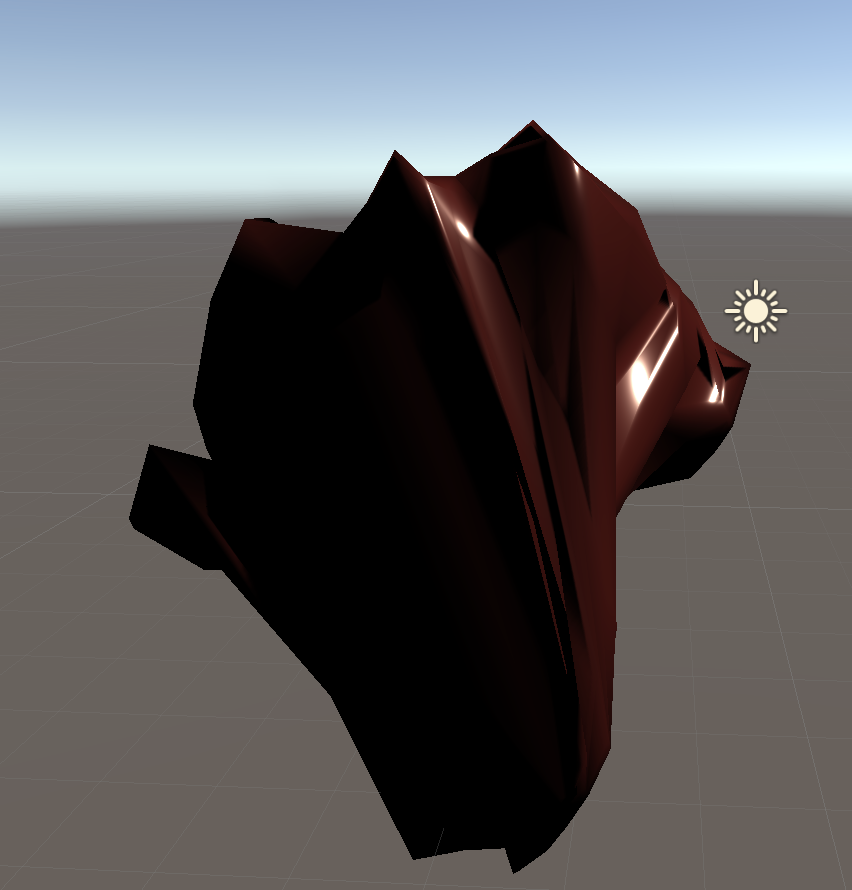
\includegraphics[width=2\columnwidth]{figures/angryobject}
  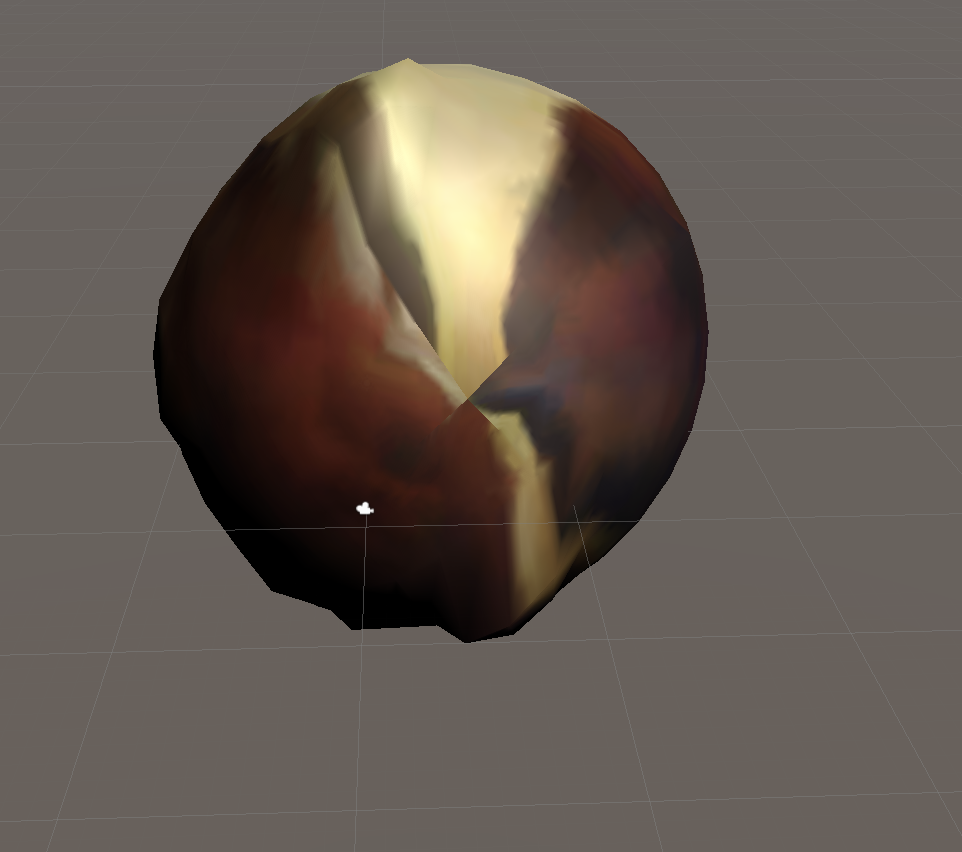
\includegraphics[width=2\columnwidth]{figures/angryGAN}
  \caption{User preference results for generated objects delineated by emotion (top). User preference for generated objects overall and process overall (bottom).}~\label{fig:figure4}
\end{figure*}

\begin{figure*}
  \centering
  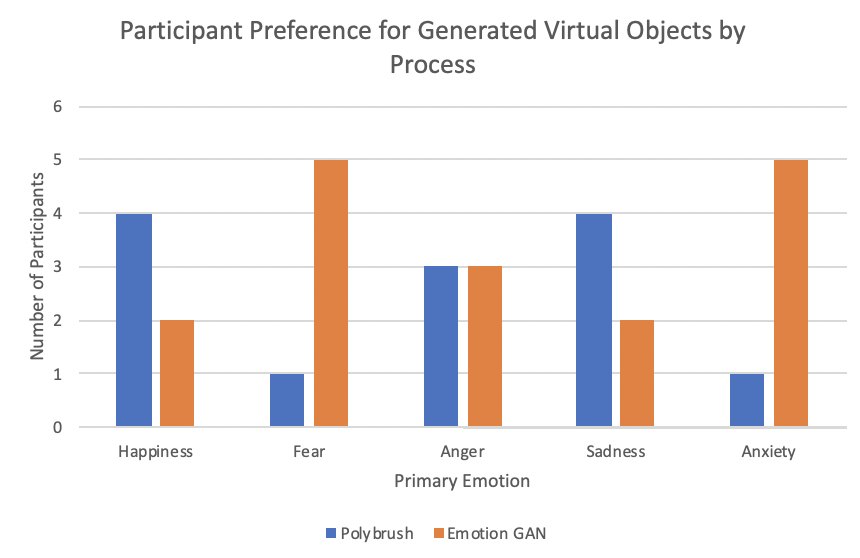
\includegraphics[width=2\columnwidth]{figures/emotiongraph}
  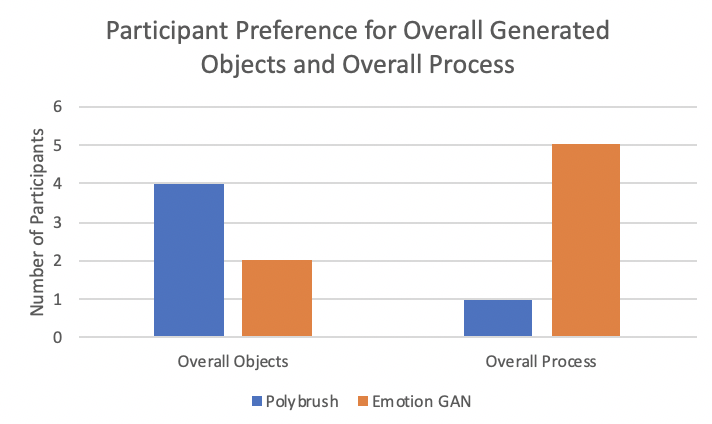
\includegraphics[width=2\columnwidth]{figures/overallgraph}
  \caption{User preference results for generated objects delineated by emotion (top). User preference for generated objects overall and process overall (bottom).}~\label{fig:figure5}
\end{figure*}

\section{Discussion}
Due to study restraints resulting from COVID-19 restrictions, we could only run the study with six participants. Thus, we were unable to provide statistically valid quantitative analysis for the study with \emph N = 6. However, to better understand the results, we conducted participant post-study surveys to garner reasoning and starting points for future studies. 

Many of the participants indicated that they preferred the polybrush created objects to the emotion GAN created ones, because they felt as if they had more control over the outcome. As one user said, “I like to make small adjustments and add lots of different colors, rather than just having the computer decide for me.” When asked about their simultaneous preference for the emotion GAN creation process, however, most participants said that it was simpler to use than the polybrush tool, and they liked the new possibilities that the GAN might create. One user also suggested that for more complex emotions like anxiety and fear, the emotion GAN also helped her “come up with a starting point” and the artistic renditions “did a better job of expressing [these] complex emotions, since [she] didn’t really know how to express that”. This user also indicated in her pre-survey that she did not usually express her emotions strongly, nor did she usually express them through creative practices.

These seemingly conflicting opinions offer some insight into the artificial intelligence co-creation process. Perhaps users would prefer more options for adjusting the final outcome of the generated image via easy-to-use interactive shaping tools or widgets, while still using the emotion GAN generated image as a starting point for creation. Similarly, offering choices for different object shapes in the emotion GAN process may provide a way for more user control in shaping the final object outcome. These may provide a basis for future studies on improving this process, but the results still suggest that our proposed generative method may provide a more accessible gateway to three-dimensional emotion-based art for many users. 

\section{Conclusion}
In this study, we have proposed a novel two-step method for generating emotion-based three-dimensional artwork from two-dimensional images and user input. Although we did not achieve state-of-the-art results, and most users preferred more control over the final representation of their generated objects, we did provide a preferred gateway for users to engage in co-creative design with artificially intelligent networks. By improving upon this process via more user input inclusion, better image generation, and three-dimensional object options, future researchers can iterate upon a viable co-creative design process for generating emotion-based three-dimensional virtual objects for creative expression and therapeutic purposes.

\section{Future Work}
In future studies, we suggest several alterations for improving and testing our proposed generative method. During the study, we only had access to a limited dataset, which resulted in less than state-of-the-art image generations from the ACGAN. As with most generative networks, the emotion based ACGAN will likely exhibit improved results if trained with larger amounts of more robust data. While we only tested five emotions separately, the neural network can easily be adjusted to generate images that represent several different emotions, or layers of emotions. For example, future research may want to test user preferences for creating objects that reflect both anger and sadness, or more complex emotions like confusion, regret, or shame. Additionally, we recommend that future researchers generate more “adjustment widgets” and object types to test user preferences for control and input during the emotion GAN process. Finally, we propose using facial recognition networks to test using facial emotions as an input method for the generative emotion GAN process, rather than user button selected emotions. While this was initially a proposed method for the study, we could not complete it due to time and situation constraints. However, we think this is a valuable avenue for generating novel input methods for the virtual creative process. These changes will generate new understandings about the human-artificial intelligence co-creative process.

\section{Acknowledgements}
Special thanks to Francisco for being a very insightful, encouraging professor and research mentor and Vidya Gaddy for her well-prepared Latex files that helped me format everything correctly.

% Use a numbered list of references at the end of the article, ordered
% alphabetically by first author, and referenced by numbers in
% brackets~\cite{ethics, Klemmer:2002:WSC:503376.503378,
%   Mather:2000:MUT, Zellweger:2001:FAO:504216.504224}. For papers from
% conference proceedings, include the title of the paper and an
% abbreviated name of the conference (e.g., for Interact 2003
% proceedings, use \textit{Proc. Interact 2003}). Do not include the
% location of the conference or the exact date; do include the page
% numbers if available. See the examples of citations at the end of this
% document. Within this template file, use the \texttt{References} style
% for the text of your citation.

% Your references should be published materials accessible to the
% public.  Internal technical reports may be cited only if they are
% easily accessible (i.e., you provide the address for obtaining the
% report within your citation) and may be obtained by any reader for a
% nominal fee.  Proprietary information may not be cited. Private
% communications should be acknowledged in the main text, not referenced
% (e.g., ``[Robertson, personal communication]'').


% Balancing columns in a ref list is a bit of a pain because you
% either use a hack like flushend or balance, or manually insert
% a column break.  http://www.tex.ac.uk/cgi-bin/texfaq2html?label=balance
% multicols doesn't work because we're already in two-column mode,
% and flushend isn't awesome, so I choose balance.  See this
% for more info: http://cs.brown.edu/system/software/latex/doc/balance.pdf
%
% Note that in a perfect world balance wants to be in the first
% column of the last page.
%
% If balance doesn't work for you, you can remove that and
% hard-code a column break into the bbl file right before you
% submit:
%
% http://stackoverflow.com/questions/2149854/how-to-manually-equalize-columns-
% in-an-ieee-paper-if-using-bibtex
%
% Or, just remove \balance and give up on balancing the last page.
%
\balance{}


% BALANCE COLUMNS
\balance{}

% REFERENCES FORMAT
% References must be the same font size as other body text.
\bibliographystyle{SIGCHI-Reference-Format}
\bibliography{sample}

\end{document}

%%% Local Variables:
%%% mode: latex
%%% TeX-master: t
%%% End:
